% Measured exhibits for Lee Ting Sen's MLR 512 project. IEEEtran template in reference/.
\RequirePackage[T1]{fontenc}
\documentclass[journal,onecolumn]{IEEEtran}
\usepackage{amsmath,graphicx,booktabs}
\usepackage[hidelinks]{hyperref}
\graphicspath{{generated/}}
\hypersetup{pdftitle={Steel Surface Inspection: Experimental Evidence for Five Detectors},pdfauthor={Lee Ting Sen}}
\newcommand{\selectedName}{stock YOLO26n}
\newcommand{\selectedID}{A}
\newcommand{\selectedSide}{480}
\newcommand{\selectedCutoff}{0.685839}
\newcommand{\headCutoff}{0.792212}
\newcommand{\matchedEvidence}{The dense head found 354 of 833 test annotations and the one-to-one head found 305. Both detected 241 of the same annotations. Dense alone found 21 rolled-in-scale boxes and one-to-one alone found 6. For scratches the corresponding counts were 7 and 23.}
\newcommand{\headFirstTitle}{Crazing, image 15, annotation 2}
\newcommand{\headSecondTitle}{Crazing, image 201, annotation 2}
\newcommand{\headCaseScores}{Score 0.814, IoU 0.603 & Score 0.770, IoU 0.611 & Score 0.788, IoU 0.622 & Score 0.840, IoU 0.564}
\newcommand{\headCaseEvidence}{On image~15, the missed crazing candidate had IoU 0.611, but its score of 0.770 fell below the alarm cutoff. On image~201, the missed crazing candidate had IoU 0.622, but its score of 0.788 fell below the alarm cutoff. Across 137 crazing annotations, 12 changed detection status when the head switched, and both heads missed 112.}
\newcommand{\selectionEvidence}{The quality and false-alarm limits admitted 1 of 5 architectures at 480 and 1 of 4 input sizes for A. The selected stock YOLO26n checkpoint (seed~0, 480 pixels) had a validation pipeline $p_{95}$ of 16.59~ms.}
\newcommand{\validationDetail}{At seed~0, A detected 43 of 85 pitted-surface objects and B detected 41. One object changes recall by 1.18~pp here. The paired mean validation mAP change for B versus A was +0.05~pp. C and D reached seed-0 validation pipeline $p_{95}$ values of 16.86 and 16.30~ms. C exceeded the seed-0 recall tolerance for patches, scratches. D exceeded the seed-0 recall tolerance for pitted surface.}
\newcommand{\trainingEvidence}{The earliest validation maxima across the fifteen runs fell between epochs 88 and 156. C reached 39.26--40.44\% validation mAP. D reached 39.53--40.48\% validation mAP. The three stock YOLO26n checkpoints provide a paired reference for these ranges.}
\newcommand{\gatePfour}{0.462--0.990}
\newcommand{\gatePthree}{0.514--0.801}
\newcommand{\fusionEvidence}{Fusion changed test mAP by -0.36~pp on stock YOLO26n and by +0.67~pp on the PConv backbone. Their paired interaction was +1.03~pp (95\% group interval [-0.55, +2.68]~pp). The interval includes zero, so these images leave the direction of the interaction uncertain. The combined detector's overall change from stock was +0.66~pp.}
\newcommand{\recoveryEvidence}{On pitted surface, PConv alone changed mean test operating recall by -1.55~pp. Adding fusion to PConv changed it by +5.81~pp, with a 95\% interval of [-0.73, +12.20]~pp. The resulting D versus A change was +4.26~pp. D regained the full observed PConv recall loss in the paired mean.}
\newcommand{\pconvTiming}{At 480 the mean B minus A change in pipeline $p_{95}$ was -0.229~ms. The paired seed differences were -0.192, +0.632 and -1.127~ms. The corresponding mAP change was -0.012~pp (95\% interval [-1.27, +1.19]~pp). Adding gates changed latency by +0.604~ms on stock and +0.351~ms on PConv.}
\newcommand{\resolutionEvidence}{On the selected architecture, moving from 480 to 320 changed mean test pipeline $p_{95}$ from 15.76 to 9.88~ms. Crazing AP50 changed by -3.68~pp and rolled-in-scale AP50 by -8.55~pp. At 256 the same weights reached 21.80\% mAP in 6.05~ms. At 640 the measurements were 27.23\% and 26.36~ms.}
\newcommand{\objectEvidence}{For the crazing annotation, the score changed from 0.729 at 320 to 0.088 at 480, with IoUs of 0.751 and 0.764. At the missed size, the class score fell below the alarm cutoff. For the rolled in scale annotation, the score changed from 0.666 at 480 to 0.842 at 640, with IoUs of 0.643 and 0.630. At the missed size, the class score fell below the alarm cutoff.}
\newcommand{\headEvidence}{Across the five OpenVINO detectors, the signed one-to-one time saving ranged from -0.241 to +0.743~ms. The signed savings for C and D were -0.241 and +0.743~ms, with mAP changes of -2.20 and -2.19~pp at the common score floor. YOLOv10n saved -0.219~ms on OpenVINO and +0.051~ms on PyTorch. Switching its OpenVINO head changed FP/image from 0.173 to 0.131.}
\newcommand{\headDiagnostics}{Standalone suppression took 0.081--0.085~ms across the model/runtime means. At seed~0 the dense and one-to-one OpenVINO head-only $p_{95}$ values for A were 1.761 and 1.982~ms. Top-$k$ selection runs inside the one-to-one graph. The dense path filters the scores of 4,725 anchors before NMS. The separate stage percentiles cannot be added to recover the full-request percentile.}
\newcommand{\runtimeEvidence}{Across two heads and three seeds, A had a lower median pipeline $p_{95}$ than E in 6 of six OpenVINO comparisons and 0 of six PyTorch comparisons. Independent annotation matching found 5 validation and 0 held-out differences between PyTorch and OpenVINO at the frozen cutoffs. Small score changes matter when an annotation lies on the alarm threshold.}
\newcommand{\selectedTiming}{The selected seed-0 checkpoint reached 70.50\% mean AP at IoU 0.50, 38.29\% mAP over IoUs 0.50--0.95, and 15.59~ms pipeline $p_{95}$. The prepared-input $p_{95}$ was 14.43~ms. The full pipeline processed 86.1 requests/s across three sessions whose pipeline $p_{95}$ ranged from 15.39 to 19.36~ms. Of the 3,000 timed requests, 433 exceeded 15~ms and 45 exceeded 20~ms.}
\newcommand{\alarmEvidence}{The selected model detected 20 of 137 crazing objects and 43 of 126 rolled-in-scale objects, at recalls of 14.6\% and 34.1\%. Their AP50 values were 42.9\% and 57.7\%. Across classes, 371 of 408 reported detections matched an annotation (90.9\% precision), and 462 of 833 annotations were missed. There were 37 false positives on 360 annotated test images (0.103 FP/image).}
\newcommand{\sizeBandEvidence}{For boxes whose shorter side measured 20 to under 50 original pixels, the model found 0 of 19 crazing and 6 of 39 rolled-in-scale objects. At 50 pixels or longer the corresponding counts were 20 of 118 and 37 of 87. A box can enclose a network of fine cracks. These box dimensions describe an annotated region and leave the minimum visible crack width undetermined.}
\newcommand{\verificationEvidence}{Two independent checks reproduced the operating counts for all 1,044 class rows, 768 paired recall intervals, and all 336 factorial interval rows. Standard COCO AP differed from the study evaluator by at most 0.0193~pp across the 174 configurations. Replaying the validation rules with standard COCO AP gave the same eligibility and selection.}
\newcommand{\reproductionEvidence}{The workspace retains split manifests, model and graph hashes, per-image detections and raw timings. The table-only report command rebuilt all 10 primary tables byte-for-byte. The runtime used Ultralytics 8.4.216, PyTorch 2.9.1 and OpenVINO 2026.4.1.}
\newcommand{\resultAbstract}{Partial convolution reduces the arithmetic cost of surface-defect detection, but its effect on CPU latency and on missed objects depends on the complete inference path. This study crossed four-site partial convolution with two image-conditioned fusion gates in YOLO26n and compared the four resulting models with YOLOv10n on NEU-DET. Each model used three matched seeds. The six gated runs extended a completed nine-run study on the same grouped split. At 480 pixels on OpenVINO, fusion changed mean average precision over intersections-over-union of 0.50--0.95 by -0.36 percentage points on stock YOLO26n and +0.67 points with partial convolution. The paired interaction was +1.03 points (95\% group interval [-0.55, +2.68]). Validation selected stock YOLO26n at 480 pixels. Its seed-0 checkpoint reached 38.29\% mean average precision and 15.59~ms 95th-percentile pipeline latency on 360 held-out images. It detected 20 of 137 crazing objects and 43 of 126 rolled-in-scale objects at the frozen alarm cutoff. The measured latency and absolute class recalls jointly qualify this operating point.}
\newcommand{\conclusionEvidence}{Under the common training and CPU protocol, the estimated fusion gain differed between the two YOLO26n backbones by +1.03~pp in test mAP. The interval includes zero, so these images leave the direction of the interaction uncertain. The joint change from stock to PConv plus fusion was +0.66~pp and +0.12~ms in pipeline $p_{95}$. The validation selection, stock YOLO26n at 480, achieved 15.59~ms pipeline $p_{95}$ while detecting 14.6\% of crazing annotations. A production trial would need a specified defect-size threshold, representative clean material, and synchronized camera-to-actuator timing.}
\newcommand{\latencySelected}{15.59}

\newcommand{\exhibit}[1]{\section*{#1}}
\newcommand{\blocktitle}[1]{\par\smallskip\noindent{\bfseries #1}\par\smallskip}
\newcommand{\fig}[2]{\begin{center}\includegraphics[width=#1\textwidth]{#2}\end{center}}
\newcommand{\tab}[1]{\begin{center}\small\input{generated/#1}\end{center}}
\newcommand{\nextpage}{\clearpage}
\begin{document}
\markboth{MLR 512, Advanced Computer Vision}{Lee Ting Sen, Five-Detector Evidence}
\title{Steel Surface Inspection on a CPU\\Experimental Evidence for Five Detectors}
\author{Lee Ting Sen\\American University of Sharjah}
\maketitle
\exhibit{Study design and grouped images}
The experiment asks whether partial convolution saves processing time, whether two learned fusion gates change its effect on quality, and how input size and detection head affect inspection. Fifteen training runs pair seeds 0, 1 and 2 across five architectures. The selected artifact is \selectedName{}, seed 0 at \selectedSide{} pixels on the OpenVINO one-to-one path.
\begin{center}\begin{tabular}{llll}
\toprule ID & Detector & PConv & Learned top-down gates\\ \midrule
A & Stock YOLO26n & No & No\\
B & YOLO26n with partial convolution & Yes & No\\
C & YOLO26n with learned fusion & No & Yes\\
D & YOLO26n with both treatments & Yes & Yes\\
E & Stock YOLOv10n & No & No\\ \bottomrule
\end{tabular}\end{center}
\blocktitle{NEU-DET annotations}
\tab{audit}
The public archive contains 1,800 grayscale images and 4,189 boxes. Grouping holds likely overlapping views together. Every architecture uses exactly the same training, validation and test manifests. The six classes are crazing, inclusion, patches, pitted surface, rolled-in scale and scratches.
\blocktitle{When the comparisons were specified}
The earlier A/B/E results were available when the six C/D runs were added. The gate definition and difference-in-differences analysis were recorded before training C or D. Nine preliminary validation sessions were archived after Windows servicing. The reported study uses a fresh 87-cell timing rotation per split. Held-out evaluation began after the expanded validation freeze.
\nextpage
\exhibit{Paired training and learned fusion}
A and B supply the ungated backbones. A gate pools each branch at the top-down P4 and P3 joins and predicts two scalar weights. Twice the softmax normalizes them to sum to two. Zero-initialized output projections start both weights at one. C matched A and D matched B exactly on both native heads at initialization for all three seeds.
\fig{.90}{training_curves.pdf}
\blocktitle{Training and checkpoint selection}
Each run used 200 epochs, a 480-pixel canvas, mixed precision, AdamW and batch 16. Loss components for YOLO26n and YOLOv10n have different definitions. All fifteen runs use the same native one-to-one validation mAP at 480 for checkpoint selection. Ties retain the earliest epoch.
\tab{training_summary}
\blocktitle{Gate weights after training}
For six validation images from each of the six image categories, the two gates of each selected C/D checkpoint produced image-dependent weights. Across all 36 images and six checkpoints, the weight on the top-down input spanned \gatePfour{} at P4 and \gatePthree{} at P3. Both hidden and output projections received finite gradients and changed weights during the first epoch.
\nextpage
\exhibit{Validation choice and measured cost}
Eligibility was checked at seed 0 and on the paired three-seed mean. At 480 pixels a candidate could lose at most 1 percentage point of mAP and 2 points of recall in any class versus A. The false-positive budget was 0.10 per annotated image. A size also had to stay within 2 points of each priority-class AP50 at its architecture's 480 reference. The table gives seed-0 measurements.
\tab{validation_decision}
\blocktitle{What the rule selected}
\selectionEvidence{}
\blocktitle{Held-out cost at 480}
\tab{architecture_cost}
Active parameters cover the selected one-to-one inference path. The FLOP counter counts two operations per multiply--accumulate for convolutions and matrix products. Pooling, branch scaling, activations, decoding, ranking and postprocessing are outside this count. Pipeline latency includes preprocessing through final boxes. AP and latency are means of the three seed estimates.
\nextpage
\exhibit{Fusion gains on the two backbones}
The primary response is mean AP over IoU 0.50--0.95 on OpenVINO at 480. The difference between the gain from B to D and the gain from A to C estimates the interaction. D minus A measures the overall effect of the combined adaptation. Each row below gives changes in percentage points and the signed change in pipeline p95 in milliseconds.
\tab{fusion}
\fig{.80}{fusion_contrasts.pdf}
\blocktitle{What happened to operating recall}
\tab{pconv_recall}
\fusionEvidence{}
\nextpage
\exhibit{Four inference sizes on the same captured pixels}
Cr and RS give crazing and rolled-in-scale AP50 in percent. The p95 column gives decoded-image-to-box latency in milliseconds. Small marks show individual seeds and connected marks show three-seed means. All four sizes use the same decoded $200\times200$ images. Each 480-pixel one-to-one graph also serves the head comparison.
\begin{center}\footnotesize\setlength{\tabcolsep}{6pt}\begin{tabular}{lrrrrr}
\hline
Model & Side & Cr AP & RS AP & mAP & p95 (ms) \\
\hline
A & 256 & 20.9 & 28.4 & 21.8 & 6.05 \\
A & 320 & 31.8 & 43.7 & 30.9 & 9.88 \\
A & 480 & 35.5 & 52.3 & 37.6 & 15.76 \\
A & 640 & 23.5 & 43.3 & 27.2 & 26.36 \\
B & 256 & 16.6 & 23.0 & 20.4 & 6.44 \\
B & 320 & 29.3 & 37.7 & 30.3 & 8.32 \\
B & 480 & 35.7 & 51.1 & 37.6 & 15.53 \\
B & 640 & 23.2 & 41.7 & 26.5 & 26.58 \\
C & 256 & 14.4 & 26.1 & 20.7 & 6.11 \\
C & 320 & 27.8 & 40.5 & 29.8 & 8.44 \\
C & 480 & 34.6 & 50.9 & 37.2 & 16.37 \\
C & 640 & 22.0 & 43.4 & 27.5 & 26.37 \\
D & 256 & 20.3 & 29.4 & 21.1 & 6.16 \\
D & 320 & 33.7 & 43.9 & 30.7 & 9.37 \\
D & 480 & 38.6 & 47.5 & 38.2 & 15.88 \\
D & 640 & 25.0 & 41.9 & 27.0 & 25.77 \\
E & 256 & 15.1 & 29.6 & 19.2 & 6.18 \\
E & 320 & 28.2 & 43.4 & 27.8 & 8.54 \\
E & 480 & 36.0 & 49.3 & 36.3 & 19.13 \\
E & 640 & 16.7 & 41.7 & 21.1 & 31.85 \\
\hline
\end{tabular}
\end{center}
\fig{.93}{test_crazing_size.pdf}
\fig{.93}{test_rolled_in_scale_size.pdf}
\nextpage
\exhibit{Two heads from one checkpoint}
OV means OpenVINO and PT means native PyTorch CPU. A positive paired saving favors one-to-one. NMS time covers suppression on filtered candidates. All other head-path differences remain inside the full-pipeline comparison. The quality delta is one-to-one minus dense in percentage points.
\tab{head_tradeoff}
\blocktitle{Which objects changed for YOLOv10n?}
\tab{yolov10_matched}
\fig{.62}{yolov10_head_cases.pdf}
Gold outlines the indicated annotation. Solid cyan marks an accepted detection. Dashed cyan marks a same-class candidate below the operating threshold. Each pair uses YOLOv10n seed 0 on the same image at 480 pixels, with a frozen cutoff of \headCutoff{}.
\nextpage
\exhibit{From a score to a matched or missed object}
The upper examples follow one annotated object across four static input sizes. Each label gives the class score and the IoU against the same original-coordinate annotation. A larger input resamples the same source pixels.
\begin{center}
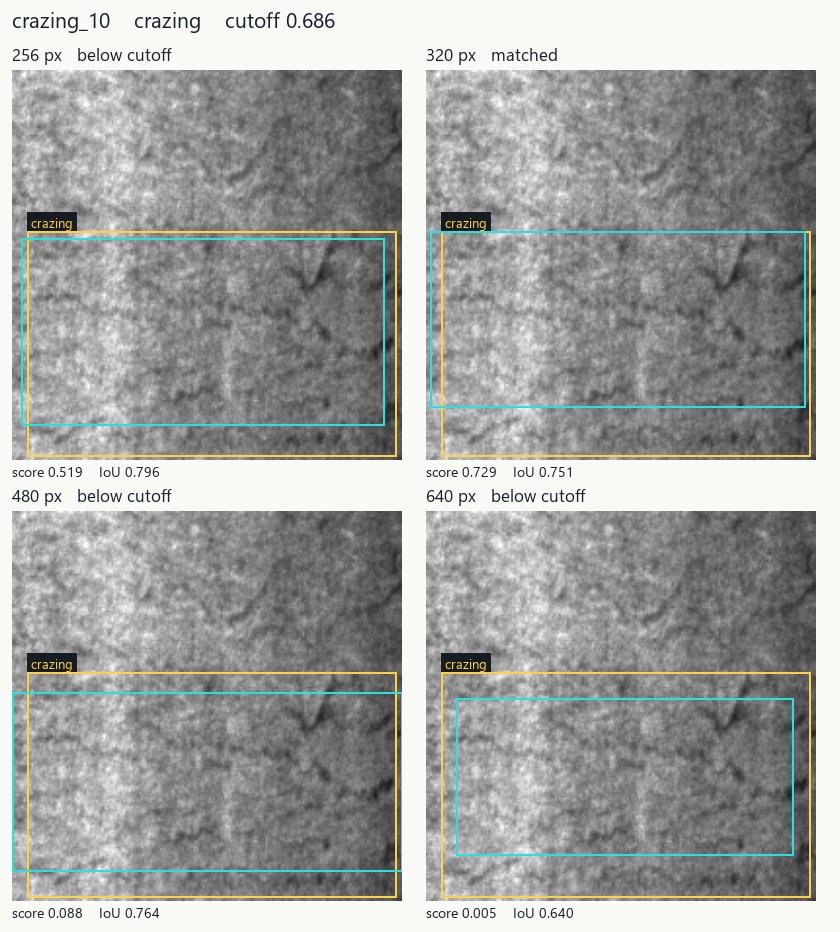
\includegraphics[width=.48\textwidth]{size_change_crazing.png}\hfill
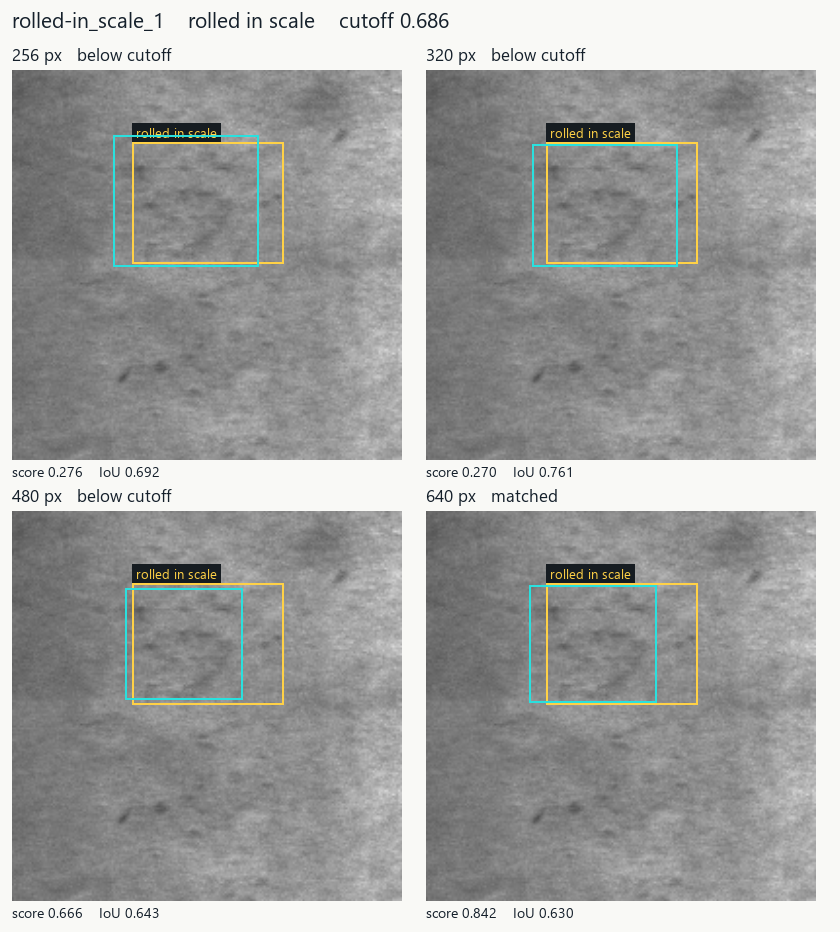
\includegraphics[width=.48\textwidth]{size_change_rolled_in_scale.png}
\end{center}
\blocktitle{Selected detector at its frozen cutoff}
\begin{center}
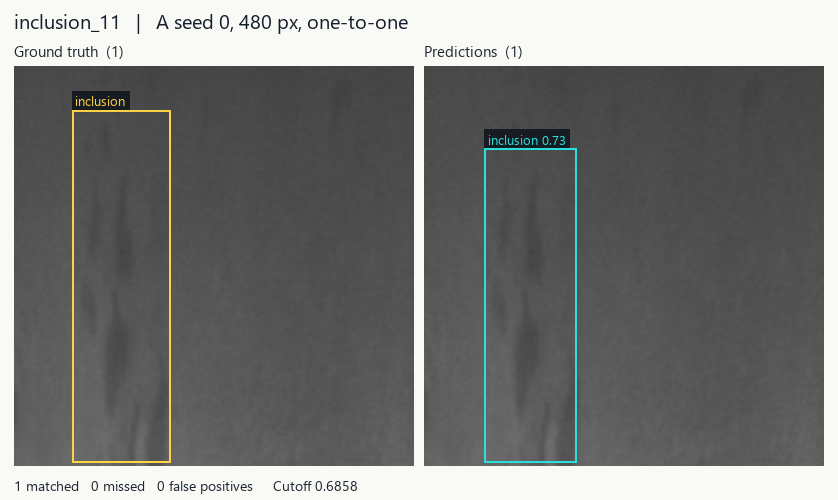
\includegraphics[width=.49\textwidth]{success.png}\hfill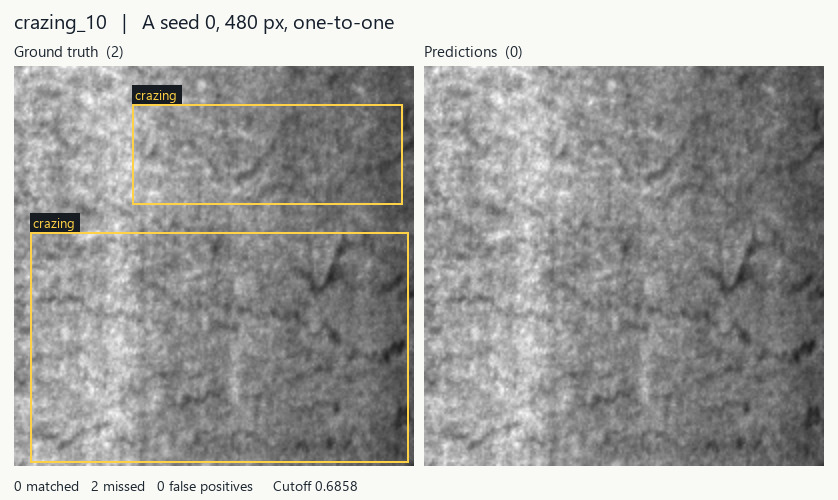
\includegraphics[width=.49\textwidth]{miss.png}\\
\smallskip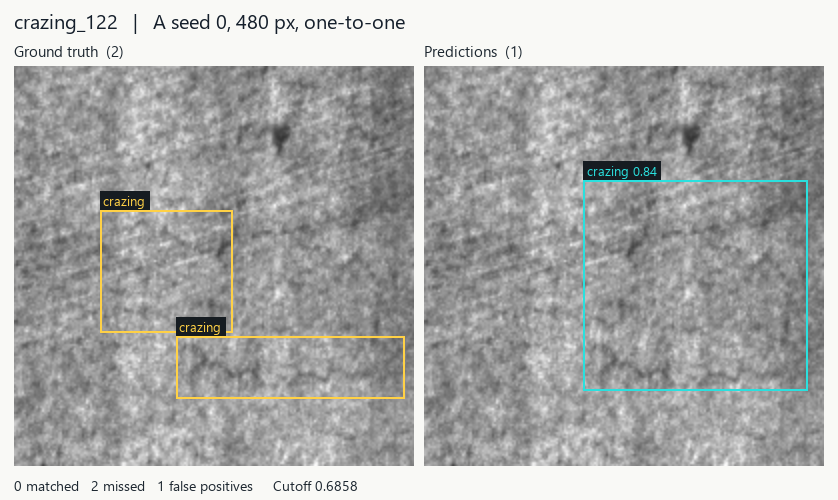
\includegraphics[width=.49\textwidth]{false_positive.png}
\end{center}
The left and right images of each pair are the original annotations and the accepted predictions. A false positive counts each unmatched detection on an annotated image.
\nextpage
\exhibit{Selected checkpoint at the alarm threshold}
Validation selected \selectedName{}, seed~0 at \selectedSide{} pixels. AP50 integrates across scores. Operating recall uses the frozen cutoff of \selectedCutoff{} and IoU of at least 0.50. Intervals use 1,000 resamples of the 334 held-out image groups.
\tab{selected_operating}
\blocktitle{Illustrative software time budgets}
\tab{latency_budgets}
Each of the three sessions contains 1,000 synchronous requests after 200 warm-ups. The interval starts with a decoded image and ends at boxes in original coordinates. A field deadline also requires camera, transport, queue and actuation measurements.
\blocktitle{Independent verification}
\verificationEvidence{}
\blocktitle{Data and methods}
The original steel data are described by He et al.~\cite{he2020}. The architecture comparisons build on FasterNet~\cite{chen2023}, steel-surface fusion experiments~\cite{yu2025}, and the YOLOv10 dual-assignment method~\cite{wang2024}. The course survey~\cite{ting2026survey} motivated the paired size and head measurements.
\bibliographystyle{IEEEtran}
\bibliography{references}
\end{document}
